% Memoria v2 (3 caras, doble columna) — plantilla uc3mmaster. Compilar desde esta carpeta: latexmk -pdf memoria_v2.tex
% Cifras: ../numeros.tex (v2, macros \dos…) y ../../final/numeros.tex (ablación de la búsqueda, común a v1 y v2).
\documentclass[memoria,twocolumn]{uc3mmaster}
\newgeometry{top=1.7cm,bottom=1.6cm,left=1.45cm,right=1.45cm,headheight=13pt,headsep=8pt,footskip=16pt}
\setlength{\columnsep}{0.6cm}
\usepackage{multirow}
\usetikzlibrary{arrows.meta,positioning}
\definecolor{azulm}{HTML}{2E6DB4}\definecolor{naranjam}{HTML}{D9731A}
\definecolor{verdem}{HTML}{2F9467}\definecolor{grism}{HTML}{5A6772}
% Generado por analisis.py: NO editar a mano.
\newcommand{\nDatasets}{12}
\newcommand{\nParticiones}{5}
\newcommand{\nCasos}{60}
\newcommand{\relRL}{0{,}96}
\newcommand{\cambioRL}{$-$4{,}4\,\%}
\newcommand{\casosRL}{36/60}
\newcommand{\dsRL}{7/12}
\newcommand{\pRL}{$1{,}000$}
\newcommand{\cambioVsEstRL}{$-$2{,}6\,\%}
\newcommand{\dsVsEstRL}{6/12}
\newcommand{\pVsEstRL}{$1{,}000$}
\newcommand{\peorDsRL}{$+$20{,}9\,\%}
\newcommand{\relKNN}{0{,}76}
\newcommand{\cambioKNN}{$-$24{,}3\,\%}
\newcommand{\casosKNN}{56/60}
\newcommand{\dsKNN}{12/12}
\newcommand{\pKNN}{$0{,}004$}
\newcommand{\cambioVsEstKNN}{$-$13{,}6\,\%}
\newcommand{\dsVsEstKNN}{10/12}
\newcommand{\pVsEstKNN}{$0{,}048$}
\newcommand{\peorDsKNN}{$-$0{,}4\,\%}
\newcommand{\relArbol}{1{,}00}
\newcommand{\cambioArbol}{$+$0{,}1\,\%}
\newcommand{\casosArbol}{34/60}
\newcommand{\dsArbol}{7/12}
\newcommand{\pArbol}{$1{,}000$}
\newcommand{\cambioVsEstArbol}{$+$0{,}1\,\%}
\newcommand{\dsVsEstArbol}{7/12}
\newcommand{\pVsEstArbol}{$1{,}000$}
\newcommand{\peorDsArbol}{$+$5{,}0\,\%}
\newcommand{\relRF}{1{,}00}
\newcommand{\cambioRF}{$+$0{,}5\,\%}
\newcommand{\casosRF}{27/60}
\newcommand{\dsRF}{5/12}
\newcommand{\pRF}{$1{,}000$}
\newcommand{\cambioVsEstRF}{$+$0{,}5\,\%}
\newcommand{\dsVsEstRF}{5/12}
\newcommand{\pVsEstRF}{$1{,}000$}
\newcommand{\peorDsRF}{$+$4{,}1\,\%}
\newcommand{\cambioSintRL}{$-$1{,}3\,\%}
\newcommand{\pSintRL}{$0{,}705$}
\newcommand{\dsSintRL}{7/12}
\newcommand{\relSintRL}{0{,}99}
\newcommand{\cambioSintKNN}{$-$0{,}3\,\%}
\newcommand{\pSintKNN}{$0{,}705$}
\newcommand{\dsSintKNN}{7/12}
\newcommand{\relSintKNN}{1{,}00}
\newcommand{\cambioSintArbol}{$+$0{,}3\,\%}
\newcommand{\pSintArbol}{$1{,}000$}
\newcommand{\dsSintArbol}{7/12}
\newcommand{\relSintArbol}{1{,}00}
\newcommand{\cambioSintRF}{$-$0{,}1\,\%}
\newcommand{\pSintRF}{$1{,}000$}
\newcommand{\dsSintRF}{7/12}
\newcommand{\relSintRF}{1{,}00}
\newcommand{\cambioRedRL}{$+$1{,}8\,\%}
\newcommand{\pRedRL}{$0{,}380$}
\newcommand{\dsRedRL}{5/12}
\newcommand{\relRedRL}{1{,}02}
\newcommand{\cambioRedKNN}{$+$1{,}0\,\%}
\newcommand{\pRedKNN}{$0{,}330$}
\newcommand{\dsRedKNN}{4/12}
\newcommand{\relRedKNN}{1{,}01}
\newcommand{\cambioRedArbol}{$+$1{,}4\,\%}
\newcommand{\pRedArbol}{$0{,}330$}
\newcommand{\dsRedArbol}{3/12}
\newcommand{\relRedArbol}{1{,}01}
\newcommand{\cambioRedRF}{$+$2{,}8\,\%}
\newcommand{\pRedRF}{$0{,}049$}
\newcommand{\dsRedRF}{1/12}
\newcommand{\relRedRF}{1{,}03}
\newcommand{\dimMedia}{83\,\%}
\newcommand{\fracEliminados}{22\,\%}
\newcommand{\dimMin}{38\,\%}
\newcommand{\dimMax}{92\,\%}
\newcommand{\mMedia}{0{,}4}
\newcommand{\fracConSintesis}{25\,\%}
\newcommand{\tauMediana}{0{,}18}
\newcommand{\casosNmenosUno}{38/60}
\newcommand{\wLat}{2{,}91}
\newcommand{\wLon}{2{,}85}
\newcommand{\wPop}{0{,}03}
\newcommand{\wInc}{0{,}41}
\newcommand{\fracApagados}{10\,\%}
\newcommand{\nCompCasos}{60}
\newcommand{\compMLKRRL}{$-$1{,}8\,\%}
\newcommand{\compMLKRKNN}{$-$22{,}5\,\%}
\newcommand{\compMLKRArbol}{$+$2{,}0\,\%}
\newcommand{\compMLKRRF}{$+$2{,}6\,\%}
\newcommand{\rangoMLKR}{5{,}7}
\newcommand{\compPGRL}{$-$15{,}7\,\%}
\newcommand{\compPGKNN}{$-$18{,}0\,\%}
\newcommand{\compPGArbol}{$+$0{,}7\,\%}
\newcommand{\compPGRF}{$+$0{,}8\,\%}
\newcommand{\rangoPG}{4{,}6}
\newcommand{\compYJMVRL}{$+$2{,}4\,\%}
\newcommand{\compYJMVKNN}{$-$14{,}5\,\%}
\newcommand{\compYJMVArbol}{$+$1{,}5\,\%}
\newcommand{\compYJMVRF}{$+$1{,}7\,\%}
\newcommand{\rangoYJMV}{5{,}0}
\newcommand{\compCuantRL}{$+$8{,}1\,\%}
\newcommand{\compCuantKNN}{$-$11{,}8\,\%}
\newcommand{\compCuantArbol}{$+$0{,}1\,\%}
\newcommand{\compCuantRF}{$+$0{,}0\,\%}
\newcommand{\rangoCuant}{6{,}4}
\newcommand{\compEstPCARL}{$-$1{,}8\,\%}
\newcommand{\compEstPCAKNN}{$-$12{,}4\,\%}
\newcommand{\compEstPCAArbol}{$-$0{,}6\,\%}
\newcommand{\compEstPCARF}{$-$1{,}9\,\%}
\newcommand{\rangoEstPCA}{4{,}6}
\newcommand{\compPCAnoventaRL}{$+$0{,}6\,\%}
\newcommand{\compPCAnoventaKNN}{$-$10{,}4\,\%}
\newcommand{\compPCAnoventaArbol}{$+$19{,}3\,\%}
\newcommand{\compPCAnoventaRF}{$+$17{,}9\,\%}
\newcommand{\rangoPCAnoventa}{8{,}1}
\newcommand{\compPCAcvRL}{$-$1{,}0\,\%}
\newcommand{\compPCAcvKNN}{$-$12{,}0\,\%}
\newcommand{\compPCAcvArbol}{$+$18{,}7\,\%}
\newcommand{\compPCAcvRF}{$+$15{,}1\,\%}
\newcommand{\rangoPCAcv}{7{,}4}
\newcommand{\compPsrRL}{$-$6{,}1\,\%}
\newcommand{\compPsrKNN}{$-$25{,}0\,\%}
\newcommand{\compPsrArbol}{$-$1{,}1\,\%}
\newcommand{\compPsrRF}{$-$2{,}3\,\%}
\newcommand{\rangoPsr}{3{,}2}
\newcommand{\compPRL}{$-$4{,}4\,\%}
\newcommand{\compPKNN}{$-$24{,}3\,\%}
\newcommand{\compPArbol}{$+$0{,}1\,\%}
\newcommand{\compPRF}{$+$0{,}5\,\%}
\newcommand{\rangoP}{4{,}7}
\newcommand{\mejorAlt}{estándar + PCA}
\newcommand{\rangoMejorAlt}{4{,}6}
\newcommand{\nReps}{10}
\newcommand{\vMedia}{0{,}80}
\newcommand{\vFracUno}{22\,\%}
\newcommand{\nSintMedia}{3{,}9}
\newcommand{\ctrlIniAleat}{$+$0{,}6\,\%}
\newcommand{\pCtrlIniAleat}{$1{,}000$}
\newcommand{\ctrlIniAleatRL}{$+$1{,}7\,\%}
\newcommand{\ctrlSigmaBajo}{$+$0{,}5\,\%}
\newcommand{\pCtrlSigmaBajo}{$1{,}000$}
\newcommand{\ctrlSigmaBajoRL}{$-$0{,}1\,\%}
\newcommand{\ctrlSigmaAlto}{$+$0{,}9\,\%}
\newcommand{\pCtrlSigmaAlto}{$1{,}000$}
\newcommand{\ctrlSigmaAltoRL}{$-$0{,}4\,\%}
\newcommand{\ctrlPobDoble}{$+$0{,}2\,\%}
\newcommand{\pCtrlPobDoble}{$1{,}000$}
\newcommand{\ctrlPobDobleRL}{$-$0{,}2\,\%}
\newcommand{\nAblCasos}{24}
\newcommand{\ctrlPesos}{$+$2{,}2\,\%}
\newcommand{\ctrlPesosRL}{$+$6{,}5\,\%}
\newcommand{\pCtrlPesos}{$0{,}424$}
\newcommand{\ctrlExp}{$+$10{,}0\,\%}
\newcommand{\ctrlExpRL}{$+$2{,}2\,\%}
\newcommand{\pCtrlExp}{$0{,}012$}
\newcommand{\ctrlAleat}{$+$6{,}2\,\%}
\newcommand{\ctrlAleatRL}{$+$3{,}0\,\%}
\newcommand{\pCtrlAleat}{$0{,}012$}
\newcommand{\ctrlMI}{$+$14{,}9\,\%}
\newcommand{\ctrlMIRL}{$+$6{,}8\,\%}
\newcommand{\pCtrlMI}{$0{,}012$}
\newcommand{\ctrlYJMI}{$+$11{,}0\,\%}
\newcommand{\ctrlYJMIRL}{$+$10{,}3\,\%}
\newcommand{\pCtrlYJMI}{$0{,}014$}
\newcommand{\nCtrlCasos}{24}
\newcommand{\rangoCeroR}{$+$2{,}2\,\%}
\newcommand{\pRangoCero}{$1{,}000$}
\newcommand{\dsPeorRangoCero}{7}
\newcommand{\rangoUnoR}{$+$0{,}3\,\%}
\newcommand{\pRangoUno}{$1{,}000$}
\newcommand{\dsPeorRangoUno}{6}
\newcommand{\rangoCuatroR}{$+$0{,}5\,\%}
\newcommand{\pRangoCuatro}{$1{,}000$}
\newcommand{\dsPeorRangoCuatro}{7}
\newcommand{\rangoOchoR}{$+$1{,}7\,\%}
\newcommand{\pRangoOcho}{$0{,}256$}
\newcommand{\dsPeorRangoOcho}{9}
\newcommand{\bordeUno}{11\,\%}
\newcommand{\bordeDos}{7\,\%}
\newcommand{\bordeCuatro}{8\,\%}
\newcommand{\bordeOcho}{5\,\%}
\newcommand{\nRango}{24}
\newcommand{\mleFueraDos}{24\,\%}
\newcommand{\nAlgCasos}{24}
\newcommand{\rangoCMA}{1{,}9}
\newcommand{\algMejor}{CMA-ES}
\newcommand{\algKNNcma}{$-$25{,}7\,\%}
\newcommand{\algKNNaleat}{$-$21{,}0\,\%}
\newcommand{\algKNNmin}{$-$24{,}8\,\%}
\newcommand{\algKNNmax}{$-$23{,}3\,\%}
\newcommand{\segMediana}{191}
\newcommand{\segMax}{243}
\newcommand{\msPorEval}{191}
\newcommand{\segMLKR}{16{,}8}
\newcommand{\segPG}{6{,}1}
\newcommand{\segYJMV}{0{,}6}
\newcommand{\popMin}{11}
\newcommand{\popMax}{13}
\newcommand{\muMin}{5}
\newcommand{\muMax}{6}
\newcommand{\muEffMin}{3{,}4}
\newcommand{\muEffMax}{4{,}0}
\newcommand{\genMin}{77}
\newcommand{\genMax}{91}
\newcommand{\nParadaPresupuesto}{12}
\newcommand{\nParadaTotal}{12}
\newcommand{\evalMejorMediana}{971}
\newcommand{\evalMejorMin}{658}
\newcommand{\mejoraFitnessMediana}{$-$12{,}1\,\%}
\newcommand{\sigmaFinMin}{0{,}007}
\newcommand{\sigmaFinMax}{0{,}06}
\newcommand{\cribSelRL}{$-$2{,}5\,\%}
\newcommand{\cribSelKNN}{$-$23{,}9\,\%}
\newcommand{\cribSelArbol}{$+$0{,}1\,\%}
\newcommand{\cribSelRF}{$+$0{,}8\,\%}
\newcommand{\cribDimSel}{72\,\%}
\newcommand{\cribFijoRL}{$-$5{,}4\,\%}
\newcommand{\cribFijoKNN}{$-$25{,}0\,\%}
\newcommand{\cribFijoArbol}{$-$0{,}5\,\%}
\newcommand{\cribFijoRF}{$+$0{,}0\,\%}
\newcommand{\cribDimFijo}{89\,\%}
\newcommand{\cribPcaRL}{$-$2{,}7\,\%}
\newcommand{\cribPcaKNN}{$-$23{,}9\,\%}
\newcommand{\cribPcaArbol}{$+$0{,}8\,\%}
\newcommand{\cribPcaRF}{$+$1{,}9\,\%}
\newcommand{\cribDimPca}{70\,\%}
\newcommand{\cribFijoNoReduce}{27/60}
% Generado por analisis.py: filas de las tablas (una macro por tabla).
\newcommand{\filasPrincipal}{%
R. lineal & 0{,}98 & 0{,}94 & \textbf{0{,}96} & 7/12 & $1{,}000$ & $-$2{,}6\,\%\\
KNN & 0{,}88 & 0{,}75 & \textbf{0{,}76} & 12/12 & $0{,}004$ & $-$13{,}6\,\%\\
Árbol & 1{,}00 & 0{,}99 & \textbf{1{,}00} & 7/12 & $1{,}000$ & $+$0{,}1\,\%\\
RF & 1{,}00 & 0{,}98 & \textbf{1{,}00} & 5/12 & $1{,}000$ & $+$0{,}5\,\%\\
}
\newcommand{\filasDimension}{%
diabetes & 10 & 8{,}0 & 0{,}6 & 8{,}6 & 0{,}46\\
concrete & 8 & 6{,}6 & 0{,}0 & 6{,}6 & 0{,}47\\
stock & 9 & 7{,}6 & 0{,}4 & 8{,}0 & 0{,}30\\
space\_ga & 6 & 3{,}8 & 0{,}4 & 4{,}2 & 0{,}09\\
sulfur & 6 & 5{,}0 & 0{,}0 & 5{,}0 & 0{,}01\\
wine\_quality & 11 & 9{,}6 & 0{,}2 & 9{,}8 & 0{,}41\\
kin8nm & 8 & 7{,}0 & 0{,}0 & 7{,}0 & 0{,}34\\
bank8FM & 8 & 6{,}8 & 0{,}2 & 7{,}0 & 0{,}05\\
puma8NH & 8 & 2{,}2 & 2{,}4 & 4{,}6 & 1{,}83\\
house\_8L & 8 & 7{,}0 & 0{,}0 & 7{,}0 & 0{,}12\\
cpu\_small & 12 & 10{,}8 & 0{,}2 & 11{,}0 & 0{,}19\\
california & 8 & 6{,}6 & 0{,}0 & 6{,}6 & 0{,}02\\
}
\newcommand{\filasComparativa}{%
estándar & 0{,}98 & 0{,}88$^*$ & 1{,}00 & 1{,}00 & 5{,}3 & 1{,}00\\
YJ máx.\ verosimilitud & 1{,}02 & 0{,}85$^*$ & 1{,}01 & 1{,}02 & 5{,}0 & 1{,}00\\
cuantiles & 1{,}08 & 0{,}88$^*$ & 1{,}00 & 1{,}00 & 6{,}4 & 1{,}00\\
solo PCA (95\,\%) & 1{,}01 & 0{,}90$^*$ & 1{,}19$^*$ & 1{,}18$^*$ & 8{,}1 & 0{,}79\\
solo PCA (\% por VC) & 0{,}99 & 0{,}88$^*$ & 1{,}19$^*$ & 1{,}15 & 7{,}4 & 0{,}91\\
estándar + su PCA & 0{,}98 & 0{,}88$^*$ & 0{,}99 & 0{,}98 & 4{,}6 & 2{,}00\\
MLKR & 0{,}98 & 0{,}78 & 1{,}02 & 1{,}03 & 5{,}7 & 1{,}00\\
PG (gplearn) & \textbf{0{,}84} & 0{,}82$^*$ & 1{,}01 & 1{,}01 & 4{,}6 & 2{,}00\\
$P$ sin reducir & 0{,}94 & \textbf{0{,}75} & \textbf{0{,}99} & \textbf{0{,}98} & 3{,}2 & 2{,}00\\
\textbf{$P$} & 0{,}96 & 0{,}76 & 1{,}00 & 1{,}00 & 4{,}7 & 0{,}83\\
}
\newcommand{\filasAblacion}{%
\multicolumn{4}{@{}l}{\emph{Piezas}}\\
\quad solo pesos ($\lambda=1$) & $+$2{,}2\,\% & $+$6{,}5\,\% & $-$0{,}1\,\%\\
\quad solo exponentes ($w=1$) & $+$10{,}0\,\%$^*$ & $+$2{,}2\,\% & $+$0{,}4\,\%\\
\midrule
\multicolumn{4}{@{}l}{\emph{Sin búsqueda}}\\
\quad pesos por inf.\ mutua & $+$14{,}9\,\%$^*$ & $+$6{,}8\,\% & $+$3{,}6\,\%\\
\quad YJ (MV) + pesos inf.\ mutua & $+$11{,}0\,\% & $+$10{,}3\,\% & $+$3{,}6\,\%\\
\midrule
\multicolumn{4}{@{}l}{\emph{Búsqueda}}\\
\quad búsqueda aleatoria (1000 puntos) & $+$6{,}2\,\%$^*$ & $+$3{,}0\,\% & $+$2{,}0\,\%\\
\midrule
\multicolumn{4}{@{}l}{\emph{Inicio}}\\
\quad media inicial aleatoria & $+$0{,}6\,\% & $+$1{,}7\,\% & $+$0{,}6\,\%\\
\quad $\sigma_0=0{,}1$ & $+$0{,}5\,\% & $-$0{,}1\,\% & $+$0{,}8\,\%\\
\quad $\sigma_0=0{,}4$ & $+$0{,}9\,\% & $-$0{,}4\,\% & $+$0{,}6\,\%\\
\quad población $\times2$ & $+$0{,}2\,\% & $-$0{,}2\,\% & $+$1{,}3\,\%\\
\midrule
\multicolumn{4}{@{}l}{\emph{Rango}}\\
\quad $\lambda\in[-1,1]$ & $+$0{,}3\,\% & $+$1{,}5\,\% & $-$0{,}3\,\%\\
\quad $\lambda\in[-4,4]$ & $+$0{,}5\,\% & $+$1{,}4\,\% & $+$1{,}1\,\%\\
\quad $\lambda\in[-8,8]$ & $+$1{,}7\,\% & $+$5{,}0\,\% & $+$1{,}4\,\%\\
}
\newcommand{\filasControles}{%
solo pesos ($\lambda=1$) & $+$2{,}2\,\% & $+$6{,}5\,\% & $-$0{,}1\,\%\\
solo exponentes ($w=1$) & $+$10{,}0\,\%$^*$ & $+$2{,}2\,\% & $+$0{,}4\,\%\\
búsqueda aleatoria & $+$6{,}2\,\%$^*$ & $+$3{,}0\,\% & $+$2{,}0\,\%$^*$\\
pesos por inf.\ mutua & $+$14{,}9\,\%$^*$ & $+$6{,}8\,\% & $+$3{,}6\,\%\\
YJ (MV) + pesos inf.\ mutua & $+$11{,}0\,\%$^*$ & $+$10{,}3\,\% & $+$3{,}6\,\%\\
}
\newcommand{\filasAlgoritmos}{%
\textbf{CMA-ES} & 1{,}9 & $-$25{,}7\,\% & $-$7{,}7\,\%\\
AG (propio) & 2{,}8 & $-$24{,}4\,\% & $-$8{,}5\,\%\\
HS & 3{,}2 & $-$24{,}5\,\% & $-$8{,}3\,\%\\
BBO & 4{,}4 & $-$24{,}8\,\% & $-$8{,}0\,\%\\
PSO & 4{,}5 & $-$24{,}1\,\% & $-$5{,}1\,\%\\
DE & 5{,}4 & $-$23{,}3\,\% & $-$5{,}9\,\%\\
ABC & 5{,}9 & $-$24{,}0\,\% & $-$2{,}4\,\%\\
búsqueda aleatoria & 7{,}9 & $-$21{,}0\,\% & $-$4{,}9\,\%\\
}
\newcommand{\filasCoste}{%
P (CMA-ES, 1000 evaluaciones) & 190{,}6 & 242{,}6\\
MLKR & 16{,}8 & 41{,}8\\
PG (gplearn) & 6{,}1 & 14{,}1\\
PCA v-CV & 1{,}0 & 11{,}5\\
YJ máx. verosimilitud & 0{,}6 & 4{,}3\\
cuantiles & 0{,}1 & 0{,}8\\
estándar + PCA & 0{,}0 & 0{,}0\\
}
\newcommand{\filasDatasets}{%
diabetes & 442 & 10\\
concrete & 1\,030 & 8\\
stock & 950 & 9\\
space\_ga & 3\,107 & 6\\
sulfur & 10\,000 & 6\\
wine\_quality & 6\,497 & 11\\
kin8nm & 8\,192 & 8\\
bank8FM & 8\,192 & 8\\
puma8NH & 8\,192 & 8\\
house\_8L & 10\,000 & 8\\
cpu\_small & 8\,192 & 12\\
california & 20\,640 & 8\\
}

% Generado por v2/analisis_v2.py: NO editar a mano.
\newcommand{\dosRelRL}{0{,}85}
\newcommand{\dosCambioRL}{$-$14{,}6\,\%}
\newcommand{\dosDsRL}{11/12}
\newcommand{\dosPRL}{$0{,}027$}
\newcommand{\dosCambioVsEstRL}{$-$13{,}1\,\%}
\newcommand{\dosPVsEstRL}{$0{,}027$}
\newcommand{\dosPeorDsRL}{$+$1{,}2\,\%}
\newcommand{\dosRelKNN}{0{,}79}
\newcommand{\dosCambioKNN}{$-$21{,}2\,\%}
\newcommand{\dosDsKNN}{9/12}
\newcommand{\dosPKNN}{$0{,}161$}
\newcommand{\dosCambioVsEstKNN}{$-$10{,}0\,\%}
\newcommand{\dosPVsEstKNN}{$0{,}386$}
\newcommand{\dosPeorDsKNN}{$+$28{,}5\,\%}
\newcommand{\dosRelArbol}{0{,}99}
\newcommand{\dosCambioArbol}{$-$0{,}6\,\%}
\newcommand{\dosDsArbol}{5/12}
\newcommand{\dosPArbol}{$1{,}000$}
\newcommand{\dosCambioVsEstArbol}{$-$0{,}7\,\%}
\newcommand{\dosPVsEstArbol}{$1{,}000$}
\newcommand{\dosPeorDsArbol}{$+$6{,}7\,\%}
\newcommand{\dosRelRF}{1{,}00}
\newcommand{\dosCambioRF}{$+$0{,}3\,\%}
\newcommand{\dosDsRF}{5/12}
\newcommand{\dosPRF}{$1{,}000$}
\newcommand{\dosCambioVsEstRF}{$+$0{,}3\,\%}
\newcommand{\dosPVsEstRF}{$1{,}000$}
\newcommand{\dosPeorDsRF}{$+$12{,}4\,\%}
\newcommand{\dosCambioMedio}{$-$9{,}5\,\%}
\newcommand{\dosCambioMedioUno}{$-$7{,}6\,\%}
\newcommand{\dosVsUnoRL}{$-$10{,}7\,\%}
\newcommand{\dosPVsUnoRL}{$0{,}010$}
\newcommand{\dosDsVsUnoRL}{11/12}
\newcommand{\dosVsUnoKNN}{$+$4{,}1\,\%}
\newcommand{\dosPVsUnoKNN}{$0{,}388$}
\newcommand{\dosDsVsUnoKNN}{4/12}
\newcommand{\dosVsUnoArbol}{$-$0{,}8\,\%}
\newcommand{\dosPVsUnoArbol}{$1{,}000$}
\newcommand{\dosDsVsUnoArbol}{6/12}
\newcommand{\dosVsUnoRF}{$-$0{,}2\,\%}
\newcommand{\dosPVsUnoRF}{$1{,}000$}
\newcommand{\dosDsVsUnoRF}{8/12}
\newcommand{\dosVsSrRL}{$-$9{,}1\,\%}
\newcommand{\dosPVsSrRL}{$0{,}014$}
\newcommand{\dosDsVsSrRL}{11/12}
\newcommand{\dosVsSrKNN}{$+$5{,}1\,\%}
\newcommand{\dosPVsSrKNN}{$0{,}192$}
\newcommand{\dosDsVsSrKNN}{3/12}
\newcommand{\dosVsSrArbol}{$+$0{,}6\,\%}
\newcommand{\dosPVsSrArbol}{$0{,}791$}
\newcommand{\dosDsVsSrArbol}{5/12}
\newcommand{\dosVsSrRF}{$+$2{,}6\,\%}
\newcommand{\dosPVsSrRF}{$0{,}259$}
\newcommand{\dosDsVsSrRF}{2/12}
\newcommand{\dosDimMedia}{83\,\%}
\newcommand{\dosDimMin}{25\,\%}
\newcommand{\dosOrigMedia}{4{,}9}
\newcommand{\dosCompMedia}{2{,}2}
\newcommand{\dosFracConComp}{93\,\%}
\newcommand{\dosSegMediana}{292}
\newcommand{\dosSegMax}{438}
\newcommand{\dosNCasos}{60}
\newcommand{\dosMaxDsRL}{cpu\_small}
\newcommand{\dosMaxRL}{$-$59{,}6\,\%}
\newcommand{\dosMaxDsKNN}{california}
\newcommand{\dosMaxKNN}{$-$58{,}7\,\%}
\newcommand{\dosMaxDsArbol}{space\_ga}
\newcommand{\dosMaxArbol}{$-$9{,}8\,\%}
\newcommand{\dosMaxDsRF}{space\_ga}
\newcommand{\dosMaxRF}{$-$11{,}7\,\%}
\newcommand{\dosMaxDs}{cpu\_small}
\newcommand{\dosMaxMod}{Regresión lineal}
\newcommand{\dosMaxCambio}{$-$59{,}6\,\%}
\newcommand{\dosMaxVsEst}{$-$59{,}6\,\%}
\newcommand{\dosMaxMae}{2{,}524}
\newcommand{\dosMaxMaeOrig}{6{,}249}
\newcommand{\dosMaxMaeEst}{6{,}249}
\newcommand{\dosRangoP}{4{,}5}
\newcommand{\dosCompPRL}{$-$14{,}6\,\%}
\newcommand{\dosCompPKNN}{$-$21{,}2\,\%}
\newcommand{\dosCompPArbol}{$-$0{,}6\,\%}
\newcommand{\dosCompPRF}{$+$0{,}3\,\%}
\newcommand{\dosRangoUno}{5{,}3}
\newcommand{\dosCompUnoRL}{$-$4{,}4\,\%}
\newcommand{\dosCompUnoKNN}{$-$24{,}3\,\%}
\newcommand{\dosCompUnoArbol}{$+$0{,}1\,\%}
\newcommand{\dosCompUnoRF}{$+$0{,}5\,\%}
\newcommand{\dosRangoSr}{3{,}6}
\newcommand{\dosCompSrRL}{$-$6{,}1\,\%}
\newcommand{\dosCompSrKNN}{$-$25{,}0\,\%}
\newcommand{\dosCompSrArbol}{$-$1{,}1\,\%}
\newcommand{\dosCompSrRF}{$-$2{,}3\,\%}
\newcommand{\dosRangoPG}{5{,}1}
\newcommand{\dosCompPGRL}{$-$15{,}7\,\%}
\newcommand{\dosCompPGKNN}{$-$18{,}0\,\%}
\newcommand{\dosCompPGArbol}{$+$0{,}7\,\%}
\newcommand{\dosCompPGRF}{$+$0{,}8\,\%}
\newcommand{\dosRangoMLKR}{6{,}5}
\newcommand{\dosCompMLKRRL}{$-$1{,}8\,\%}
\newcommand{\dosCompMLKRKNN}{$-$22{,}5\,\%}
\newcommand{\dosCompMLKRArbol}{$+$2{,}0\,\%}
\newcommand{\dosCompMLKRRF}{$+$2{,}6\,\%}
\newcommand{\dosRangoEstPCA}{5{,}2}
\newcommand{\dosCompEstPCARL}{$-$1{,}8\,\%}
\newcommand{\dosCompEstPCAKNN}{$-$12{,}4\,\%}
\newcommand{\dosCompEstPCAArbol}{$-$0{,}6\,\%}
\newcommand{\dosCompEstPCARF}{$-$1{,}9\,\%}
\newcommand{\dosRangoYJMV}{5{,}6}
\newcommand{\dosCompYJMVRL}{$+$2{,}4\,\%}
\newcommand{\dosCompYJMVKNN}{$-$14{,}5\,\%}
\newcommand{\dosCompYJMVArbol}{$+$1{,}5\,\%}
\newcommand{\dosCompYJMVRF}{$+$1{,}7\,\%}
\newcommand{\dosRangoPCA}{8{,}9}
\newcommand{\dosCompPCARL}{$+$0{,}6\,\%}
\newcommand{\dosCompPCAKNN}{$-$10{,}4\,\%}
\newcommand{\dosCompPCAArbol}{$+$19{,}3\,\%}
\newcommand{\dosCompPCARF}{$+$17{,}9\,\%}
\newcommand{\dosPosicionP}{2}
\newcommand{\dosNReps}{11}
\newcommand{\dosCribCasos}{12}
\newcommand{\dosCribUno}{0{,}912}
\newcommand{\dosCribUnoSeg}{103}
\newcommand{\dosCribUnoEval}{1000}
\newcommand{\dosCribMulti}{0{,}887}
\newcommand{\dosCribMultiSeg}{172}
\newcommand{\dosCribMultiEval}{1002}
\newcommand{\dosCribParada}{0{,}902}
\newcommand{\dosCribParadaSeg}{71}
\newcommand{\dosCribParadaEval}{441}
\newcommand{\dosCribParadaTreinta}{0{,}897}
\newcommand{\dosCribParadaTreintaSeg}{87}
\newcommand{\dosCribParadaTreintaEval}{792}
\newcommand{\dosCribSeleccion}{0{,}895}
\newcommand{\dosCribSeleccionSeg}{98}
\newcommand{\dosCribSeleccionEval}{1002}
% Generado por v2/analisis_v2.py.
\newcommand{\filasPrincipalDos}{%
R. lineal & 0{,}98 & 0{,}94 & 0{,}96 & \textbf{0{,}85} & 11/12 & $0{,}027$\\
KNN & 0{,}88 & 0{,}75 & 0{,}76 & \textbf{0{,}79} & 9/12 & $0{,}161$\\
Árbol & 1{,}00 & 0{,}99 & 1{,}00 & \textbf{0{,}99} & 5/12 & $1{,}000$\\
RF & 1{,}00 & 0{,}98 & 1{,}00 & \textbf{1{,}00} & 5/12 & $1{,}000$\\
}
\newcommand{\filasDimensionDos}{%
diabetes & 10 & 6{,}2 & 2{,}8 & 9{,}0\\
concrete & 8 & 5{,}8 & 1{,}0 & 6{,}8\\
stock & 9 & 6{,}4 & 1{,}6 & 8{,}0\\
space\_ga & 6 & 2{,}8 & 2{,}2 & 5{,}0\\
sulfur & 6 & 3{,}0 & 2{,}0 & 5{,}0\\
wine\_quality & 11 & 7{,}0 & 3{,}0 & 10{,}0\\
kin8nm & 8 & 4{,}6 & 2{,}4 & 7{,}0\\
bank8FM & 8 & 3{,}6 & 3{,}4 & 7{,}0\\
puma8NH & 8 & 2{,}2 & 0{,}6 & 2{,}8\\
house\_8L & 8 & 5{,}4 & 1{,}6 & 7{,}0\\
cpu\_small & 12 & 7{,}2 & 3{,}8 & 11{,}0\\
california & 8 & 5{,}0 & 2{,}0 & 7{,}0\\
}
\newcommand{\filasComparativaDos}{%
estándar & 0{,}98$^*$ & 0{,}88 & 1{,}00 & 1{,}00 & 5{,}9 & 1{,}00\\
YJ máx.\ verosimilitud & 1{,}02$^*$ & 0{,}85 & 1{,}01 & 1{,}02 & 5{,}6 & 1{,}00\\
cuantiles & 1{,}08$^*$ & 0{,}88 & 1{,}00 & 1{,}00 & 7{,}0 & 1{,}00\\
solo PCA (95\,\%) & 1{,}01$^*$ & 0{,}90 & 1{,}19$^*$ & 1{,}18 & 8{,}9 & 0{,}79\\
solo PCA (\% por VC) & 0{,}99$^*$ & 0{,}88 & 1{,}19$^*$ & 1{,}15 & 8{,}3 & 0{,}91\\
estándar + su PCA & 0{,}98$^*$ & 0{,}88 & 0{,}99 & 0{,}98 & 5{,}2 & 2{,}00\\
MLKR & 0{,}98$^*$ & 0{,}78 & 1{,}02 & 1{,}03 & 6{,}5 & 1{,}00\\
PG (gplearn) & \textbf{0{,}84} & 0{,}82 & 1{,}01 & 1{,}01 & 5{,}1 & 2{,}00\\
$P$ sin reducir & 0{,}94$^*$ & \textbf{0{,}75} & \textbf{0{,}99} & \textbf{0{,}98} & 3{,}6 & 2{,}00\\
$P$ v1 & 0{,}96$^*$ & 0{,}76 & 1{,}00 & 1{,}00 & 5{,}3 & 0{,}83\\
\textbf{$P$ v2} & 0{,}85 & 0{,}79 & 0{,}99 & 1{,}00 & 4{,}5 & 0{,}83\\
}
\newcommand{\filasCribadoDos}{%
$P$ v1 (fitness KNN) & 0{,}98 & 0{,}70 & 0{,}99 & 1{,}02 & 0{,}912 & 1000 & 103\\
\textbf{KNN+RL+árbol} & 0{,}89 & 0{,}72 & 0{,}96 & 1{,}00 & 0{,}887 & 1002 & 172\\
\quad + parada (pac.\ 15) & 0{,}90 & 0{,}73 & 0{,}99 & 1{,}02 & 0{,}902 & 441 & 71\\
\quad + parada (pac.\ 30) & 0{,}89 & 0{,}73 & 0{,}98 & 1{,}01 & 0{,}897 & 792 & 87\\
\quad + elegir $\theta$ con apartado & 0{,}89 & 0{,}73 & 0{,}98 & 1{,}01 & 0{,}895 & 1002 & 98\\
pesos dobles, KNN + parada & 0{,}96 & 0{,}72 & 0{,}98 & 1{,}01 & 0{,}911 & 468 & 30\\
}


\titulo{Transformación evolutiva de atributos v2}
\asignatura{IA con inspiración biológica}
\autor{Andrea López Salazar}{}
\graphicspath{{../figuras/}{../../final/figuras/}}
\captionsetup{font=footnotesize,skip=3pt}
\setlength{\textfloatsep}{7pt plus 2pt}
\setlength{\floatsep}{5pt plus 2pt}
\setlength{\dbltextfloatsep}{7pt plus 2pt}
\titlespacing*{\section}{0pt}{0.9ex plus .3ex}{0.4ex}
\titlespacing*{\subsection}{0pt}{0.7ex plus .2ex}{0.25ex}
\setlength{\parskip}{2pt plus 1pt}

\begin{document}
\twocolumn[{%
\begin{tikzpicture}[remember picture,overlay,every node/.style={anchor=west,text=white,font=\sffamily}]
  \fill[uc3mazul] (current page.north west) rectangle ([yshift=-3.0cm]current page.north east);
  \fill[uc3mcian] ([yshift=-3.0cm]current page.north west) rectangle ([yshift=-3.1cm]current page.north east);
  \node[font=\sffamily\scriptsize\bfseries] at ([xshift=1.45cm,yshift=-0.75cm]current page.north west)
     {MEMORIA \textbullet\ IA CON INSPIRACIÓN BIOLÓGICA \textbullet\ MÁSTER EN CIENCIA Y TECNOLOGÍA \textbullet\ UC3M};
  \node[font=\sffamily\Large\bfseries] at ([xshift=1.45cm,yshift=-1.5cm]current page.north west)
     {Aumentar, ponderar y reducir: transformación evolutiva de atributos};
  \node[font=\sffamily\small] at ([xshift=1.45cm,yshift=-2.35cm]current page.north west) {Andrea López Salazar};
  \node[font=\sffamily\small,anchor=east] at ([xshift=-1.45cm,yshift=-2.35cm]current page.north east)
     {Curso 2026--2027};
\end{tikzpicture}
\vspace*{1.05cm}
\begin{resultado}[Resumen]\small
Aprendemos con CMA-ES, solo con el entrenamiento, una transformación $X\!\to\!X'$ con menos atributos que $X$.
Primero se \emph{aumenta}: a cada atributo, con su forma corregida (Yeo-Johnson), se le añaden las componentes
principales, y cada uno de los $2n$ candidatos recibe su propio peso. Después se \emph{reduce}: se conservan los de
peso mayor que un umbral que aprende la evolución, como mucho $n-1$. El fitness es la media del error normalizado de
KNN, regresión lineal y un árbol. En \nDatasets{} datasets $\times$ \nParticiones{} particiones no usadas para
diseñarla, $X'$ usa el \dosDimMedia{} de los atributos y el error baja en regresión lineal (\dosCambioRL, \dosDsRL{}
datasets, significativo) y en KNN (\dosCambioKNN); en los árboles queda igual. Frente a la versión con fitness solo de
KNN, la regresión lineal mejora un \dosVsUnoRL{} más, a costa de \dosVsUnoKNN{} en KNN. Es la mejor de las
transformaciones que no aumentan la dimensión. Una parada por sobreajuste con datos apartados no mejoró el resultado.
\end{resultado}
\vspace{1pt}}]

\section{Problema y método}
El enunciado pide un programa $P$ que, viendo solo $(X_t,y_t)$, haga \textbf{síntesis y reducción de la
dimensionalidad} ($\dim X'<n$, con un criterio de eliminación que dependa del algoritmo evolutivo) y consiga que un
modelo \emph{arbitrario} $M$ entrenado con $X'_t$ tenga menor MAE en validación ($e'<e$). KNN es sensible a la
geometría; la regresión lineal (RL), a la forma de cada atributo; los árboles solo a las \emph{direcciones} por las que
cortan. Nuestra primera versión (v1), con fitness solo de KNN, cumplía $\dim X'<n$ y mejoraba mucho a KNN
(\cambioKNN), pero no a RL ni a los árboles. La v2 cambia dos cosas (Fig.~\ref{fig:esquema}):

\textbf{Aumentar y luego reducir.} (1) \emph{Forma}: $\tilde x_j=(\psi(x_j;\lambda_j)-\mu_j)/\sigma_j$, con
Yeo-Johnson $\lambda_j\in[-2,2]$. (2) \emph{Aumentar}: $2n$ candidatos $c=[\tilde x_1..\tilde x_n\mid p_1..p_n]$, con
$p$ las componentes principales de $\tilde x$ estandarizadas (calculadas antes de ponderar: sin dependencia circular y
baratas). (3) \emph{Pesos dobles}: cada candidato se multiplica por su peso $v_k\in[0,3]$. (4) \emph{Reducir}: se
conservan los de $v_k\ge\tau$; si son $n$ o más, los $n-1$ de mayor peso. Así $\dim X'\le n-1$ para todo individuo.

\textbf{Criterio de eliminación evolutivo.} El individuo es $\theta=(\lambda,v,\tau)$, $3n+1$ genes reales: CMA-ES
decide qué candidatos sobreviven (originales o componentes, por su peso) y cuántos ($\tau\in[0,3]$).
\textbf{Fitness de varios modelos}: media del MAE de validación cruzada (5 pliegues) de KNN ($k=5$), RL y un árbol de
decisión, cada uno dividido por el MAE de predecir la mediana, en hasta 2000 filas del entrenamiento. El árbol hace de
sustituto barato de Random Forest (RF), que solo se mide al final. Un árbol es invariante a la forma y a los pesos de
cada atributo: su término solo premia elegir bien qué componentes entran.

\begin{figure}[t]
\centering\def\esquemaescala{0.6}
% Esquema de P v2 (aumentar -> ponderar -> reducir), compartido por memoria, paper y póster de v2.
% Requiere tikz con arrows.meta y positioning; colores azulm, naranjam, verdem, grism.
\providecommand{\esquemaescala}{1}
\begin{tikzpicture}[scale=\esquemaescala, every node/.style={transform shape},
  node distance=3.5mm and 4mm,
  caja/.style={draw=azulm, rounded corners=2pt, fill=azulm!8, align=center, inner sep=2.5pt,
               minimum height=9mm, font=\footnotesize},
  sint/.style={caja, draw=verdem, fill=verdem!10},
  red/.style={caja, draw=naranjam, fill=naranjam!8},
  fl/.style={-{Stealth[length=2mm]}, thick, azulm!80!black},
  fv/.style={fl, verdem!80!black},
  fn/.style={fl, naranjam!80!black}]
\node (x) {$X$};
\node[caja, right=of x] (yj) {1. Forma\\$\psi(x_j;\lambda_j)$, estandarizar};
\node[sint, right=of yj] (aum) {2. Aumentar ($2n$)\\$c=[\,\tilde x_1..\tilde x_n \mid p_1..p_n\,]$};
\node[caja, below=7mm of aum] (pes) {3. Pesos dobles\\$v_k\,c_k$,\; $k=1..2n$};
\node[red, left=of pes] (red) {4. Reducir\\$v_k\ge\tau$, como mucho $n-1$};
\node[draw=grism, thick, rounded corners=2pt, fill=white, font=\footnotesize, minimum height=7mm,
      left=of red] (xp) {$X'$,\; $\dim X'<n$};
\draw[fl] (x)--(yj); \draw[fv] (yj)--(aum); \draw[fl] (aum)--(pes); \draw[fn] (pes)--(red); \draw[fn] (red)--(xp);
\node[font=\scriptsize\itshape, text=grism, align=left, anchor=west] at ([xshift=8mm]aum.east)
     {$p$: componentes\\principales de $\tilde x$};
\coordinate (r) at ([xshift=5mm]aum.east);
\node[caja, draw=naranjam, fill=naranjam!10, above=6mm of yj.north east, anchor=south, align=center] (cma)
     {CMA-ES busca $\theta=(\lambda,v,\tau)$ ($3n+1$ genes) minimizando la media del MAE normalizado\\
      de validación cruzada de \textbf{KNN, regresión lineal y árbol} en el entrenamiento};
\draw[fn] (cma.south -| yj) -- (yj.north);
\draw[fn] (cma.south -| r) -- (r |- pes.east) -- (pes.east);
\end{tikzpicture}

\caption{$P$ v2. CMA-ES aprende la forma, un peso para cada uno de los $2n$ candidatos y el umbral $\tau$; la
decodificación garantiza $\dim X'\le n-1$.}
\label{fig:esquema}
\end{figure}

\textbf{Diseño evolutivo.} CMA-ES parte de $\mathcal N(\theta_0,\sigma_0^2I)$ en $[0,1]^D$ con $\sigma_0=0{,}2$ y
$\theta_0$ = estandarizar sin componentes ($\lambda=1$, $v_{\text{orig}}=1$, $v_{\text{comp}}=0$, $\tau=0{,}5$).
Cada generación muestrea $4+\lfloor3\ln D\rfloor$ candidatos y selecciona por \emph{rango} la mitad mejor (invariante a
transformaciones monótonas del fitness y robusta al ruido de la validación cruzada); la nueva media es su media
ponderada (recombinación intermedia) y la mutación $\mathcal N(m,\sigma^2C)$ adapta $\sigma$ y la covarianza $C$, que
aprende qué genes se mueven juntos. Reemplazo $(\mu/\mu_w,\lambda)$ generacional guardando el mejor evaluado; parada a
las 1000 evaluaciones.

\section{Protocolo}
Doce datasets de regresión: diabetes y california (práctica) y diez de OpenML (6--12 atributos, $\le$10\,000 filas).
\textbf{Dos fases}: las variantes de v2 se compararon en un \emph{cribado} con semillas de exploración (0--1, 6
datasets); la elegida se \emph{confirma} en particiones 70/30 nuevas (semillas 40--44), las mismas de la v1, así que
todas las comparaciones son pareadas. \textbf{Modelos fijos}: RL, KNN ($k=5$), árbol y RF (100 árboles), por defecto.
\textbf{Estadística por dataset} (n=12): media geométrica de $e'/e$; Wilcoxon con Holm; Friedman y Nemenyi.

\section{Resultados}
\subsection{Diseño de v2: el cribado}
\begin{table}[t]\centering\scriptsize\setlength{\tabcolsep}{2.2pt}
\caption{Cribado (\dosCribCasos{} particiones de exploración): $e'/e$ por modelo y medio, evaluaciones y segundos
por búsqueda. Negrita: la variante elegida.}
\label{tab:cribado}
\begin{tabular}{@{}lccccccc@{}}\toprule
Variante & RL & KNN & Árbol & RF & media & eval. & s\\\midrule
\filasCribadoDos\bottomrule
\end{tabular}
\end{table}
El fitness de varios modelos mejora la media de los cuatro modelos (\dosCribMulti{} frente a \dosCribUno{} de la v1;
Tabla~\ref{tab:cribado}). \textbf{Parar por sobreajuste no ayudó}: apartar un 20\,\% de la submuestra, evaluar ahí el
mejor de cada generación y parar si no mejora en 15 generaciones reduce el tiempo de \dosCribMultiSeg{} a
\dosCribParadaSeg\,s, pero empeora (\dosCribParada). Con más paciencia (\dosCribParadaTreinta) o usando lo apartado
solo para elegir el $\theta$ final, sin parar (\dosCribSeleccion), tampoco se recupera: el coste no está en cuándo se
para, sino en quitar datos al fitness para un criterio de 60--400 filas, demasiado ruidoso para decidir.

\begin{figure*}[t]
\centering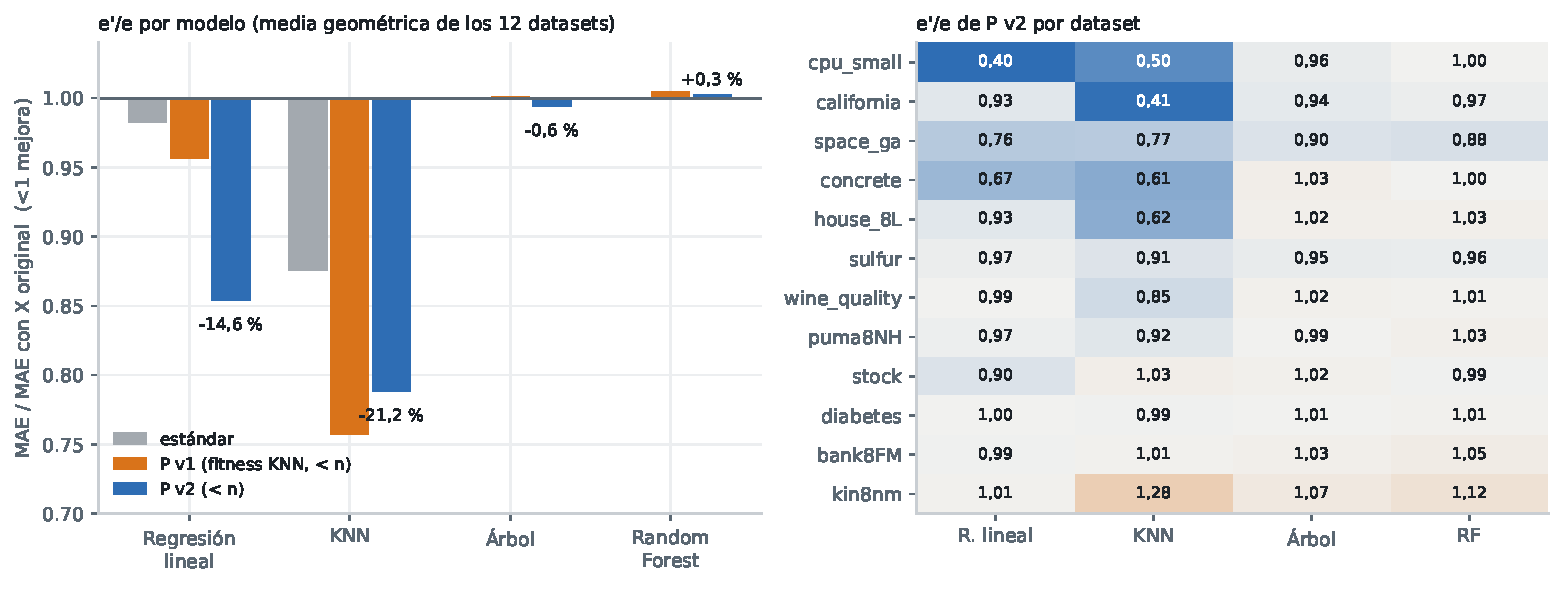
\includegraphics[width=0.86\textwidth]{principal_v2}
\caption{Izquierda: $e'/e$ por modelo para $X$ estandarizado, $P$ v1 (fitness KNN) y $P$ v2. Derecha: $e'/e$ de $P$
v2 por dataset (azul: mejora; naranja: empeora).}
\label{fig:principal}
\end{figure*}

\subsection{Criterio del enunciado}
\begin{table}[t]\centering\footnotesize\setlength{\tabcolsep}{2.3pt}
\caption{$e'/e$ (media geométrica de 12 datasets). \emph{Datasets}: con $e'<e$; $p$: Wilcoxon por dataset con Holm,
$P$ v2 frente a $X$ original.}
\label{tab:principal}
\begin{tabular}{@{}lcccccc@{}}\toprule
Modelo & estándar & sin red.\ ($2n$) & $P$ v1 & $P$ v2 & Datasets & $p$\\\midrule
\filasPrincipalDos\bottomrule
\end{tabular}
\end{table}
Con $\dim X'<n$ (Tabla~\ref{tab:principal}, Fig.~\ref{fig:principal}), la RL mejora \dosCambioRL{} (\dosDsRL{}
datasets, $p=$\dosPRL), \dosVsUnoRL{} más que con la v1 ($p=$\dosPVsUnoRL): las componentes y la forma elegidas también
para un modelo lineal le sirven. KNN mejora \dosCambioKNN{} (\dosDsKNN{}), algo menos que con la v1 (\dosVsUnoKNN, no
significativo) y ya sin significación tras Holm, porque en kin8nm empeora un \dosPeorDsKNN. En el árbol (\dosCambioArbol)
y en RF (\dosCambioRF) no hay cambio en media, aunque hay datasets donde ganan (space\_ga: RF \dosMaxRF). En media de
los cuatro modelos, la v2 mejora un \dosCambioMedio{} frente a \dosCambioMedioUno{} de la v1. La \textbf{mayor
reducción} es en \dosMaxDsRL{} con RL (\dosMaxRL; el MAE pasa de \dosMaxMaeOrig{} a \dosMaxMae) y en
\dosMaxDsKNN{} con KNN (\dosMaxKNN).

\subsection{La reducción de dimensionalidad}
\begin{table}[t]\centering\footnotesize\setlength{\tabcolsep}{4pt}
\caption{Reducción aprendida (media de 5 particiones): $n$ atributos, originales y componentes conservados y $\dim X'$.}
\label{tab:dimension}
\begin{tabular}{@{}lcccc@{}}\toprule
Dataset & $n$ & originales & componentes & $\dim X'$\\\midrule
\filasDimensionDos\bottomrule
\end{tabular}
\end{table}
$X'$ usa de media el \dosDimMedia{} de los atributos (Tabla~\ref{tab:dimension}): \dosOrigMedia{} originales y
\dosCompMedia{} componentes. A diferencia de la v1, que casi nunca sintetizaba, la v2 conserva componentes en el
\dosFracConComp{} de las particiones: el fitness de varios modelos sí reparte el presupuesto de $n-1$ atributos entre
originales y direcciones oblicuas. En puma8NH, donde pocos atributos explican $y$, se queda con 3 de 8. El reparto
falla en kin8nm, donde todos los atributos importan por igual: cambiar originales por componentes empeora a los cuatro
modelos.

\subsection{Comparativa con otras transformaciones}
\begin{table}[t]\centering\footnotesize\setlength{\tabcolsep}{2.2pt}
\caption{Comparativa: $e'/e$ (negrita: mejor; $^*$: $P$ v2 mejor con $p<0{,}05$, Wilcoxon por dataset con Holm), rango
medio de Friedman sobre los cuatro modelos y $d/n=\dim X'/n$.}
\label{tab:comparativa}
\begin{tabular}{@{}lcccccc@{}}\toprule
Transformación & R.\ lin. & KNN & Árbol & RF & Rango & $d/n$\\\midrule
\filasComparativaDos\bottomrule
\end{tabular}
\end{table}
En las mismas particiones (Tabla~\ref{tab:comparativa}), $P$ v2 es \textbf{segunda en rango medio} (\dosRangoP), solo
por detrás de $P$ sin reducir (\dosRangoSr, $2n$ atributos), y la \textbf{mejor de las que no aumentan la dimensión}:
supera a la v1 (\dosRangoUno), a la programación genética (\dosRangoPG, $2n$ atributos), a añadir la PCA de $X$
estandarizado y a MLKR. En RL es significativamente mejor que todas salvo la programación genética, con la que empata.
``Solo PCA'', la otra forma de reducir, empeora a RF un \dosCompPCARF{} (Fig.~\ref{fig:rf}): sustituir los ejes
originales por componentes daña a los árboles; \emph{elegir} cuáles conservar, no.

\begin{figure}[t]\centering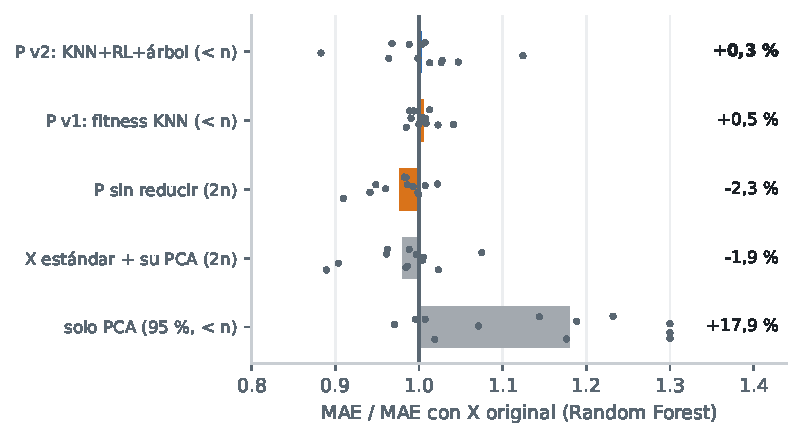
\includegraphics[width=\columnwidth]{rf_v2}
\caption{Random Forest en las mismas particiones. Punto: dataset; barra: media geométrica.}
\label{fig:rf}
\end{figure}

\subsection{La búsqueda: piezas, inicio, rango y algoritmo}
\begin{table}[t]\centering\footnotesize\setlength{\tabcolsep}{4pt}
\caption{Ablación de la búsqueda de $(\lambda,w)$, común a v1 y v2: cambio del MAE frente a CMA-ES en \nAblCasos{}
particiones ($>0$: peor; $^*$: $p<0{,}05$ por dataset, Holm).}
\label{tab:ablacion}
\begin{tabular}{@{}lccc@{}}\toprule
Variante & KNN & R.\ lineal & RF\\\midrule
\filasAblacion\bottomrule
\end{tabular}
\end{table}
La Tabla~\ref{tab:ablacion} cambia una decisión de la búsqueda de forma y pesos cada vez. Los \textbf{pesos} son la
pieza principal (sin ellos KNN empeora \ctrlExp), la búsqueda gana a la aleatoria con el mismo presupuesto
(\ctrlAleat) y a los pesos por información mutua (\ctrlMI), y CMA-ES es robusto a la población inicial y al rango de
$\lambda$. Con el mismo fitness y presupuesto, CMA-ES tiene el mejor rango de fitness (\rangoCMA) entre siete
optimizadores, aunque AG, HS y BBO quedan cerca: la búsqueda importa; el algoritmo concreto, bastante menos.

\subsection{Coste y casos negativos}
Una búsqueda de v2 tarda \dosSegMediana\,s de mediana por partición con 20 procesos en paralelo (la v1, \segMediana\,s):
el árbol y la RL encarecen cada evaluación. Se paga una sola vez por dataset y $X'$ tiene menos columnas que $X$.
Casos negativos: kin8nm (todos los atributos importan; la v2 los sustituye por componentes) y diabetes (309 filas: la
búsqueda mejora el fitness, no la validación).

\section{Conclusiones}
\begin{itemize}
\item \textbf{$\dim X'<n$ siempre} (\dosDimMedia{} de los atributos), con el criterio de eliminación aprendido por
CMA-ES, y \textbf{síntesis real}: la v2 conserva componentes en el \dosFracConComp{} de las particiones.
\item \textbf{$e'<e$ en media para RL} (\dosCambioRL, significativo) \textbf{y KNN} (\dosCambioKNN); los árboles quedan
igual en media. Mejor media de los cuatro modelos que la v1 (\dosCambioMedio{} frente a \dosCambioMedioUno).
\item \textbf{El fitness decide para quién es la representación}: con KNN sola, la v1 favorecía a KNN; con tres
modelos, la v2 reparte y gana sobre todo en RL, a costa de algo de KNN.
\item \textbf{Mejor transformación de las que no aumentan la dimensión} y segunda en rango medio entre once.
\item \textbf{La parada con datos apartados no compensa} con estos tamaños: quita datos al fitness y su criterio es
demasiado ruidoso.
\item \textbf{Límites}: 12 datasets pequeños; casos negativos (kin8nm, diabetes); $\sim$5 minutos por búsqueda; a los
árboles les ayuda sobre todo \emph{añadir} dimensiones, lo que el enunciado no permite.
\end{itemize}

{\footnotesize\textbf{Reproducibilidad.} \texttt{v2/metodo\_v2.py} (programa $P$), \texttt{cribado\_v2.py},
\texttt{experimento\_v2.py}, \texttt{analisis\_v2.py} y \texttt{notebook\_v2.ipynb} (todo el proceso, ejecutable).\par}
\end{document}
